\documentclass[12pt,a4paper,final]{article}
\usepackage[latin1]{inputenc}
\usepackage[numbers]{natbib}  % default authoryear
\usepackage[T1]{fontenc}
\usepackage{amsmath}
\usepackage{amsfonts}
\usepackage{amssymb}
\usepackage{setspace}
\usepackage[pagewise]{lineno}
\usepackage{graphicx,epstopdf}
\usepackage{subfigure}
\usepackage[verbose,a4paper,tmargin=2.4cm,bmargin=2.4cm,lmargin=2.4cm,rmargin=2.4cm]{geometry}
\usepackage[hidelinks]{hyperref}
\usepackage{url}
\usepackage[multiple]{footmisc}
\usepackage{setspace}


% Use the PLoS provided bibtex style
%\bibliographystyle{plos2009}

\usepackage{color,ulem} % package for text color comments

\author{Vasilis Dakos and Leo Lahti}

\title{
\begin{figure}[h]
%\begin{left}

\includegraphics[scale=0.55]{logoEWS.eps}
%\end{left}
\end{figure}
Early Warning Signals Toolbox:\\ 
A novel approach for Detecting Critical Transitions\\
Part 5 - Additional Information
%{\small 
%Part 5 - Additional Information
%}
}

\begin{document}
\maketitle

\begin{doublespacing}

\section{List of Relevant Publications}
Here we include the 5 most relevant publications to our submission. Despite that they have appeared only in the last years, they have already a high impact on the scientific community.\\
\\
$[1]$ M. Scheffer, S. R. Carpenter, T. M. Lenton, J. Bascompte, W. Brock, V. Dakos, J. van de Koppel, I. A. van de Leemput, S. A. Levin, E. H. van Nes, M. Pascual, and J. Vandermeer. Anticipating Critical Transitions. Science, 338(6105):344 - 348, 2012.\\
\textit{This paper summarizes the developments on the research of critical transitions, highlighting the big steps done and the challenges ahead. It also introduces the necessity and value of our toolbox.}\\
\\
$[2]$ V. Dakos, S. R. Carpenter, W. A. Brock, A. M. Ellison, V. Guttal, A. R. Ives, S. K\'{e}fi, V. Livina, D. A. Seekell, E. H. van Nes, and M. Scheffer. Methods for detecting early warnings of critical transitions in time series illustrated using simulated ecological data. PLoS ONE,
7(7):e41010, 2012.\\
\textit{This paper demonstrates how to implement and interpret most of the existing methods and indicators of signaling approaching transitions. It is a methodological paper that supports the approaches described in our toolbox.}\\
\\
$[3]$  L. Dai, D. Vorselen, K. S. Korolev, and J. Gore. Generic Indicators for Loss of Resilience Before a Tipping Point Leading to Population Collapse. Science, 336(6085):1175 - 1177,  2012.\\
\textit{This paper is an excellent demonstration of the phenomenon of critical slowing down and its signatures as expected by theory. It is based on experimental data of yeast culture in the lab.}\\
\\
$[4]$ M. Scheffer, J. Bascompte, W. A. Brock, V. Brovkin, S. R. Carpenter, V. Dakos, H. Held, E. H. van Nes, M. Rietkerk, and G. Sugihara. Early-warning signals for critical transitions. Nature, 461(7260):53 - 59, 2009.\\
\textit{This paper is the ground-breaking perspective on early-warnings for critical transitions. It is a review that summarized the theory and the potential applications that have found ground in recent years.}\\
\\
$[5]$ V. Dakos, M. Scheffer, E. H. van Nes, V. Brovkin, V. Petoukhov, and H. Held. Slowing down as an early warning signal for abrupt climate change. Proceedings of the National Academy
of Sciences of the United States of America, 105(38):14308 - 12, 2008.\\
\textit{This paper is the first paper that captured early-warning signals in time series of past climatic transitions. It introduced the first methods for measuring indicators of critical slowing down as well as conjectured the existence of tipping points in the climate.}

\newpage
\section{Web Resource}
As stated in our submission, the Early Warning Signals Toolbox comes together with a webpage (\url{www.early-warning-signals.org}) that provides background information, summarizes methods, presents case studies%\footnote{\url{www.early-warning-signals.org/?page_id=17}}
, and offers latest updates on the science and application%\footnote{\url{www.early-warning-signals.org/?p=790}}
. Clearly, this research and the corresponding methods are only now started to emerge. This webpage serves as inventory and a quick-start guide for scientists, practitioners and policy-makers who want to understand how complex systems work and to adopt new methods in their work.

\begin{figure}[ht]
%begin{center}
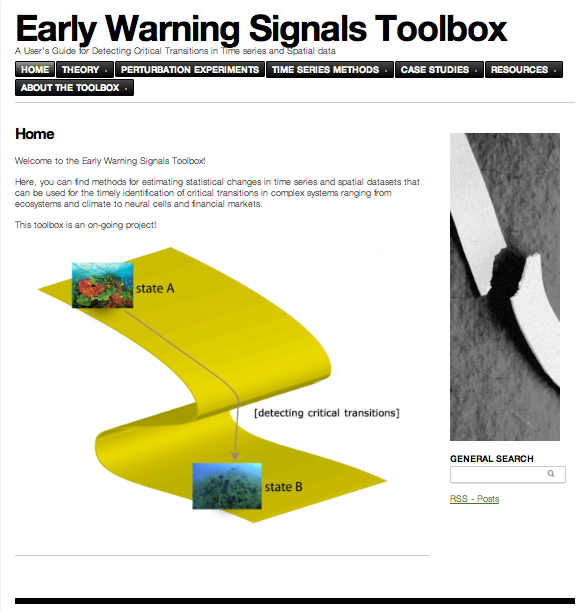
\includegraphics[scale=0.8]{webpage_ews_home.png}
%\end{center}
\end{figure}

\end{doublespacing}


\end{document}

